% ==== Document Class & Packages =====
\documentclass[12pt,hidelinks]{article}
	\usepackage[explicit]{titlesec}
	\usepackage{titletoc}
	\usepackage{tocloft}
	\usepackage{charter}
	\usepackage[many]{tcolorbox}
	\usepackage{amsmath}
	\usepackage{graphicx}
	\graphicspath{{images/}}
	\usepackage{listings}
	\usepackage{xcolor}
	\usepackage{tikz,lipsum,lmodern}
	\usetikzlibrary{calc}
	\usepackage[english]{babel}
	\usepackage{fancyhdr}
	\usepackage{mathrsfs}
	\usepackage{empheq}
	\usepackage{fourier}% change to lmodern if fourier is no available
	\usepackage{wrapfig}
	\usepackage{fancyref}
	\usepackage{hyperref}
	\usepackage{cleveref}
	\usepackage{listings}
	\usepackage{varwidth}
	\usepackage{longfbox}
	\usepackage{geometry}
	\usepackage{marginnote}
	\tcbuselibrary{theorems}
	\tcbuselibrary{breakable, skins}
	\tcbuselibrary{listings, documentation}
	\geometry{
		a4paper,
		left=33mm,
		right=33mm,
		top=20mm}
% ========= Path to images ============
%   - Direct the computer on the path 
% 	  to the folder containg the images
% =====================================
\graphicspath{{./images/}}
% ============= Macros ================
\newcommand{\fillin}{\underline{\hspace{.75in}}{\;}}
\newcommand{\solution}{\textcolor{mordantred19}{Solution:}}
\setlength{\parindent}{0pt}
\addto{\captionsenglish}{\renewcommand*{\contentsname}{Table of Contents}}
\linespread{1.2}
% ======== Footers & Headers ==========
\cfoot{\thepage}
\chead{}\rhead{}\lhead{}
% =====================================
\renewcommand{\thesection}{\arabic{section}}
\newcommand\sectionnumfont{% font specification for the number
	\fontsize{380}{130}\color{myblueii}\selectfont}
\newcommand\sectionnamefont{% font specification for the name "PART"
	\normalfont\color{white}\scshape\small\bfseries }
% ============= Colors ================
% ----- Red -----
\definecolor{mordantred19}{rgb}{0.68, 0.05, 0.0}
% ----- Blue -----
\definecolor{st.patrick\'sblue}{rgb}{0.14, 0.16, 0.48}
\definecolor{teal}{rgb}{0.0, 0.5, 0.5}
\definecolor{beaublue}{rgb}{0.74, 0.83, 0.9}
\definecolor{mybluei}{RGB}{0,173,239}
\definecolor{myblueii}{RGB}{63,200,244}
\definecolor{myblueiii}{RGB}{199,234,253}
% ---- Yellow ----
\definecolor{blond}{rgb}{0.98, 0.94, 0.75}
\definecolor{cream}{rgb}{1.0, 0.99, 0.82}
% ----- Green ------
\definecolor{emerald}{rgb}{0.31, 0.78, 0.47}
\definecolor{darkspringgreen}{rgb}{0.09, 0.45, 0.27}
% ---- White -----
\definecolor{ghostwhite}{rgb}{0.97, 0.97, 1.0}
\definecolor{splashedwhite}{rgb}{1.0, 0.99, 1.0}
% ---- Grey -----
\definecolor{whitesmoke}{rgb}{0.96, 0.96, 0.96}
\definecolor{lightgray}{rgb}{0.92, 0.92, 0.92}
\definecolor{floralwhite}{rgb}{1.0, 0.98, 0.94}
% ========= Part Format ==========
\titleformat{\section}
{\normalfont\huge\filleft}
{}
{20pt}
{\begin{tikzpicture}[remember picture,overlay]
	\fill[myblueiii] 
	(current page.north west) rectangle ([yshift=-13cm]current page.north east);   
\node[
	fill=mybluei,
	text width=2\paperwidth,
	rounded corners=6cm,
	text depth=18cm,
	anchor=center,
	inner sep=0pt] at (current page.north east) (parttop)
	{\thepart};%
\node[
	anchor=south east,
	inner sep=0pt,
	outer sep=0pt] (partnum) at ([xshift=-20pt]parttop.south) 
	{\sectionnumfont\thesection};
\node[
	anchor=south,
	inner sep=0pt] (partname) at ([yshift=2pt]partnum.south)   
	{\sectionnamefont SECTION};
\node[
	anchor=north east,
	align=right,
	inner xsep=0pt] at ([yshift=-0.5cm]partname.east|-partnum.south) 
	{\parbox{.7\textwidth}{\raggedleft#1}};
\end{tikzpicture}%
}
% ========= Hyper Ref ===========
\hypersetup{
	colorlinks,
	linkcolor={red!50!black},
	citecolor={blue!50!black},
	urlcolor={blue!80!black}
}
% ========= Example Boxes =============
\tcbset{
	defstyle/.style={
		fonttitle=\bfseries\upshape, 
		fontupper=\slshape,
		arc=0mm, 
		beamer,
		colback=blue!5!white,
		colframe=blue!75!black},
	theostyle/.style={
		fonttitle=\bfseries\upshape, 
		fontupper=\slshape,
		colback=red!10!white,
		colframe=red!75!black},
	visualstyle/.style={
		height=6.5cm,
		breakable,
		enhanced,
		leftrule=0pt,
		rightrule=0pt,
		bottomrule=0pt,
		outer arc=0pt,
		arc=0pt,
		colframe=mordantred19,
		colback=lightgray,
		attach boxed title to top left,
		boxed title style={
			colback=mordantred19,
			outer arc=0pt,
			arc=0pt,
			top=3pt,
			bottom=3pt,
		},
		fonttitle=\sffamily,},
	discussionstyle/.style={
		height=6.5cm,
		breakable,
		enhanced,
		rightrule=0pt,
		toprule=0pt,
		outer arc=0pt,
		arc=0pt,
		colframe=mordantred19,
		colback=lightgray,
		attach boxed title to top left,
		boxed title style={
			colback=mordantred19,
			outer arc=0pt,
			arc=0pt,
			top=3pt,
			bottom=3pt,
		},
		fonttitle=\sffamily},
	mystyle/.style={
		height=6.5cm,
		breakable,
		enhanced,
		rightrule=0pt,
		leftrule=0pt,
		bottomrule=0pt,
		outer arc=0pt,
		arc=0pt,
		colframe=mordantred19,
		colback=lightgray,
		attach boxed title to top left,
		boxed title style={
			colback=mordantred19,
			outer arc=0pt,
			arc=0pt,
			top=3pt,
			bottom=3pt,
		},
		fonttitle=\sffamily},
	aastyle/.style={
			height=3.5cm,
			enhanced,
			colframe=teal,
			colback=lightgray,
			colbacktitle=floralwhite,
			fonttitle=\bfseries,
			coltitle=black,
		attach boxed title to top center={
	  		yshift=-0.25mm-\tcboxedtitleheight/2,
	   		yshifttext=2mm-\tcboxedtitleheight/2}, 
		boxed title style={boxrule=0.5mm,
			frame code={ \path[tcb fill frame] ([xshift=-4mm]frame.west)
				-- (frame.north west) -- (frame.north east) -- ([xshift=4mm]frame.east)
				-- (frame.south east) -- (frame.south west) -- cycle; },
			interior code={ 
				\path[tcb fill interior] ([xshift=-2mm]interior.west)
				-- (interior.north west) -- (interior.north east)
				-- ([xshift=2mm]interior.east) -- (interior.south east) -- (interior.south west)
				-- cycle;} }
				},
	examstyle/.style={
		height=9.5cm,
		breakable,
		enhanced,
		rightrule=0pt,
		leftrule=0pt,
		bottomrule=0pt,
		outer arc=0pt,
		arc=0pt,
		colframe=mordantred19,
		colback=lightgray,
		attach boxed title to top left,
		boxed title style={
			colback=mordantred19,
			outer arc=0pt,
			arc=0pt,
			top=3pt,
			bottom=3pt,
		},
		fonttitle=\sffamily},
	doc head command={
		interior style={
			fill,
			left color=yellow!20!white, 
			right color=white}},
	doc head environment={
		boxsep=4pt,
		arc=2pt,
		colback=yellow!30!white,
		},
	doclang/environment content=text
}
% ============= Boxes ================
\newtcolorbox[auto counter,number within=section]{example}[1][]{
	mystyle,
	title=Example~\thetcbcounter,
	overlay unbroken and first={
		\path
		let
		\p1=(title.north east),
		\p2=(frame.north east)
		in
		node[anchor=
			west,
			font=\sffamily,
			color=st.patrick\'sblue,
			text width=\x2-\x1] 
		at (title.east) {#1};
	}
}
\newtcolorbox[auto counter,number within=section]{longexample}[1][]{
	examstyle,
	title=Example~\thetcbcounter,
	overlay unbroken and first={
		\path
		let
		\p1=(title.north east),
		\p2=(frame.north east)
		in
		node[anchor=
		west,
		font=\sffamily,
		color=st.patrick\'sblue,
		text width=\x2-\x1] 
		at (title.east) {#1};
	}
}
\newtcolorbox[auto counter,number within=section]{example2}[1][]{
	aastyle,
	title=Example~\thetcbcounter,{}
}
\newtcolorbox[auto counter,number within=section]{discussion}[1][]{
	discussionstyle,
	title=Discussion~\thetcbcounter,
	overlay unbroken and first={
		\path
		let
		\p1=(title.north east),
		\p2=(frame.north east)
		in
		node[anchor=
		west,
		font=\sffamily,
		color=st.patrick\'sblue,
		text width=\x2-\x1] 
		at (title.east) {#1};
	}
}
\newtcolorbox[auto counter,number within=section]{visualization}[1][]{
	visualstyle,
	title=Visualization~\thetcbcounter,
	overlay unbroken and first={
		\path
		let
		\p1=(title.north east),
		\p2=(frame.north east)
		in
		node[anchor=
		west,
		font=\sffamily,
		color=st.patrick\'sblue,
		text width=\x2-\x1] 
		at (title.east) {#1};
	}
}
% --------- Theorems ---------
\newtcbtheorem[number within=subsection,crefname={definition}{definitions}]%
	{Definition}{Definition}{defstyle}{def}%
\newtcbtheorem[use counter from=Definition,crefname={theorem}{theorems}]%
	{Theorem}{Theorem}{theostyle}{theo}
	%
\newtcbtheorem[use counter from=Definition]{theo}{Theorem}%
{
	theorem style=plain,
	enhanced,
	colframe=blue!50!black,
	colback=yellow!20!white,
	coltitle=red!50!black,
	fonttitle=\upshape\bfseries,
	fontupper=\itshape,
	drop fuzzy shadow=blue!50!black!50!white,
	boxrule=0.4pt}{theo}
\newtcbtheorem[use counter from=Definition]{DashedDefinition}{Definition}%
 {
 	enhanced,
 	frame empty,
 	interior empty,
 	colframe=darkspringgreen!50!white,
	coltitle=darkspringgreen!50!black,
	fonttitle=\bfseries,
	colbacktitle=darkspringgreen!15!white,
	borderline={0.5mm}{0mm}{darkspringgreen!15!white},
	borderline={0.5mm}{0mm}{darkspringgreen!50!white,dashed},
	attach boxed title to top center={yshift=-2mm},
	boxed title style={boxrule=0.4pt},
	varwidth boxed title}{theo}
%%%%%%%%%%%%%%%%%%%%%%%%%%%%%%%%%%%%%%%%
\newtcblisting[auto counter,number within=section]{disexam}{
	skin=bicolor,
	colback=white!30!beaublue,
	colbacklower=white,
	colframe=black,
	before skip=\medskipamount,
	after skip=\medskipamount,
	fontlower=\footnotesize,
	listing options={style=tcblatex,texcsstyle=*\color{red!70!black}},}
%%%%%%%%%%%%%%%%%%%%%%%%%%%%%%%%%%%%%%%

\begin{document}
\begin{titlepage}
	\centering % Center everything on the title page
	\scshape % Use small caps for all text on the title page
	\vspace*{1.5\baselineskip} % White space at the top of the page
% ===================
%	Title Section 	
% ===================

	\rule{13cm}{1.6pt}\vspace*{-\baselineskip}\vspace*{2pt} % Thick horizontal rule
	\rule{13cm}{0.4pt} % Thin horizontal rule
	
		\vspace{0.75\baselineskip} % Whitespace above the title
% ========== Title ===============	
	{	\Huge Manual en R in \LaTeX \\	}
% ======================================
		\vspace{0.75\baselineskip} % Whitespace below the title
	\rule{13cm}{0.4pt}\vspace*{-\baselineskip}\vspace{3.2pt} % Thin horizontal rule
	\rule{13cm}{1.6pt} % Thick horizontal rule
	
		\vspace{1.75\baselineskip} % Whitespace after the title block
% =================
%	Information	
% =================
	{\large Realizado por: \begin{itemize}
	    \item \textbf{Glenn NIcolas Rico} 
	    \item \textbf{Maykoll Gil}
	    \item \textbf{Miguel Angel Barrera }
	\end{itemize}
		\vspace*{1.2\baselineskip}
	\textbf{glennn.ricol@konradlorenz.edu.co} \vspace{2mm}\\
	miguela.gomezb@konradlorenz.edu.co \vspace{2mm}\\
	maykollj.gilm@konradlorenz.edu.co} \\
	\vfill

\end{titlepage}
%%%%%%%%%%%%%%%%%%%%%%%%%%%%%%%%%%%%%%%%%%%%%%%%%%%
\lstset{language=R,
		    basicstyle=\small\ttfamily,
		    stringstyle=\color{DarkGreen},
		    otherkeywords=[0,1,2,3,4,5,6,7,8,9],
		    morekeywords={TRUE,FALSE},
		    deletekeykeywords={data,frame,length,as,character},
		    keywordstyle=\color{blue},
		    commentstyle=\color{DarkGreen},
}
%%%%%%%%%%%%%%%%%%%%%%%%%%%%%%%%%%%%%%%%%%%%%%%%%%%%%%%%%%%
\tableofcontents
\vfill
\small{\noindent \textbf{About This File} \vspace{-3mm}\\
\noindent \rule{3.3cm}{0.5pt} \\
This file was created for the benefit of all teachers and students wanting to use Latex for tests/exams/lessons/thesis/articles etc.\\
The entirety of the contents within this file, and folder, are free for public use.}
\newpage
\newgeometry{
	left=29mm, 
	right=29mm, 
	top=20mm, 
	bottom=15mm}
%%%%%%%%%%%%%%%%%%%%%%%%%%%%%%%%%%%%%%%%%%%%%%%%%%%%%%%%%%%
\section{Brief Introduction to Latex}
\vspace{10.5cm}
	LaTeX, which is pronounced «Lah-tech» or «Lay-tech», is a document preparation system for high-quality typesetting. It is most often used for medium-to-large technical or scientific documents but it can be used for almost any form of publishing.\\
	When using Latex, \textbf{\emph{make sure to keep your source code organized by indenting and using sections/chapters/subsections}}. Not keeping your source code organized makes it harder to fix possible errors in your code.
	\subsection{Downloading Tex Studio}
			Latex is free to download and is available on all types of operating systems. To download \LaTeX, click the url to the right:\, \url{https://www.texstudio.org/}
	\subsection{Source Code and Resume Templates}
			If interested in obtaining the source code for this guide, see:\\
			\url{https://sourceforge.net/p/latex-source-code/wiki/Download/}\\
			If interested in obtaining some of the resume templates I have created, see:\\ \url{https://sourceforge.net/p/latex-resume-template/wiki/download/}
	\subsection{LaTeX Files}
			LaTeX files have names that end with the extension .tex: for example, an acceptable file name might be myfile.tex. (Never use spaces in file names.) The input file contains both the text of your document and the LATEX commands needed to format it. The first command in the file, \cs{documentclass}, defines the style of the document.
	\subsubsection{LaTeX Commands}
			To distinguish them from text, all LATEX commands (also called control sequences) start with a backslash \cs. A command name consists of letters only and is ended by a space or a non letter.
	\subsection{General Items}
		\begin{docCommand}{usepackage}{}
			Packages in latex allow for the user to include cool and unique features into ones document. Most packages for latex will be found on \url{www.ctan.org}
			\begin{verbatim}
				\usepackage{package}
			\end{verbatim}
		\end{docCommand}
	\subsection{Terminology to Know}
			\begin{itemize}
				\item Preamble:\, All the code that precedes your \cs{begin}\brackets{document}. The preamble section of your document is where all the formatting takes place. 
				\item Commands:\, Commands are special words that determine \LaTeX behavior.
				\item Environments:\, Environments are used to format blocks of text in a \LaTeX documents
			\end{itemize}
	\subsection{Tex Studio Commands}
		\begin{itemize}
			\item The button with the magnifying glass, labeled view, in the top part of Tex Studio allows you to view your document sidebyside with your code.
			\item The green arrows next to the magnifying class, labeled compile, allows you to update your document with any new code you include. Compiling also allows you to check if there are any errors in your code.  
		\end{itemize}
	\subsection{Creating Templates}
		One of the many great things about \LaTeX\ is that offers many ways to avoid some of the repetitive things that come with creating several documents. One of the features \LaTeX\ offers is to create personal user templates for files that a user often uses but does not want to continuously type out every time.\\
		For example, lets say you wanted to save a general layout of a lesson document that included \textbf{both} the preamble and some of the actual text and commands in the document. 
		To create the template, one would first proceed to the folder originally containing this pdf (The Contents You Downloaded from the Zip File)) and then go to the folder labeled \textbf{Files to make Templates out of}. Once there, click the file named: \textbf{Lesson Template}. Once you have opened that file in texstudio, go to \textbf{File}, then \textbf{Make Template}. Once that is done, give the template a name and then press ok.\\
		After creating a template, all a user needs to do to use that template is to go back to \textbf{File}, and then \textbf{New From Template} and then click the template you created.
	\vspace{-1.5mm}
\newpage
%%%%%%%%%%%%%%%%%%%%%%%%%%%%%%%%%%%%%%%%%%%%%%%%%%%%%%%%%%%
\section{Including and Inputing other Files}
\vspace{10.5cm}
	\begin{docCommand}{input}{\brackets{\sl{file-name}}}
		Imports the commands from filename.tex into the target file; it's equivalent to typing all the commands from filename.tex right into the current file where the \cs{input} line is. 
	\end{docCommand}
	\begin{docCommand}{include}{\brackets{\sl{file-name}}}
		The \cs{include} macro is bigger and is supposed to be used with bigger amounts of content, like chapters, which people might like to compile on their own during the editing process.
	\end{docCommand}
\paragraph{}If you would like to get a better understanding on the difference between the \cs{include} vs \cs{input} command, then I would suggest checking out the following website:
\begin{center}
\url{https://tex.stackexchange.com/questions/246/when-should-i-use-input-vs-include}    
\end{center}
\newpage
%%%%%%%%%%%%%%%%%%%%%%%%%%%%%%%%%%%%%%%%%%%%%%%%%%%%%%%%%%%
\section{Probabilidad}
\vspace{10.5cm}
La probabilidad es simplemente qué tan posible es que ocurra un evento determinado cuando interviene el azar.
	\subsection{Condicionada} 
	    La probabilidad condicionada mide la probabilidad de un determinado suceso conociendo información previa sobre otro suceso.
	    
	    Dado dos sucesos \textbf{A} y \textbf{B} tales que \textbf{B $\neq$ 0}, se denomina probabilidad de \textbf{A} condicionada de \textbf{B} que se escribe \textbf{P(A$/$B)}, definida:
	    
	    \begin{center}
	        \textbf{$P(A/B)=\frac{P(A\cap B)}{P(A)}$}
	    \end{center}
	    De la fórmula de la probabilidad condicionada se puede derivar una expresión que nos resulta:
	    \begin{center}
	        \textbf{P(A$\cap$B)=P(A/B)$\cdot$P(A)}
	    \end{center}
	    Esta es la expresión llamada principio de la probabilidad compuesta.
	    
	    Ejemplo vamos a calcular la probabilidad
	    del rango en el lanzamiento de 3 dados de tres formas diferentes.
		\begin{lstlisting}
		    # primera forma
            rango.dados1<- function(n){
              b1<-matrix(0,n,3)
              b1<-sapply(1:n,function(x){sample(1:6,3,T)})
              r<-apply(b1,2,max)-apply(b1, 2, min)
              prob<-table(r)/n
              return(prob)
            }
            rango.dados1(100)
        \end{lstlisting} 
        Para ejecutar este código tenemos en cuenta las aplicaciones de \textbf{apply}, \textbf{table} y se va a ejecutar en 100 pasos y el resultado sera de la siguiente manera.
        \\
            \centering
            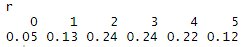
\includegraphics[scale=0.4]{probabilidad_condicionada.jpeg}\\
            \centering
            \caption{}\\
        Ahora vamos a utilizar la siguiente linea de código para calcular los vectores usando las simulaciones.\\
            
        \begin{lstlisting}
            # segunda forma 
            rango.dados2<- function(n){
              b1<-rep(0,n)
              for (i in 1:n) {
                  b1[i]= diff(range(sample(1:6,3,T)))
                }
              prob<-table(b1)/n
              return(b1)
            }
            rango.dados2(100)
        \end{lstlisting}
        El código debería ejecutado debería ejecutar lo siguiente:\\
        
            \centering
            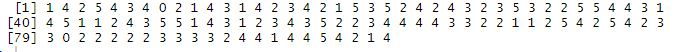
\includegraphics[scale=1]{probabilidad_condicionada1.JPG}
            \centering
            \caption{}
        \\
        Y por ultimo la ultima sentencia de código que vamos a utilizar va hacer de la siguiente manera \\
        \begin{lstlisting}
            # tercera forma
            rango.dados3<-function(n){
              b1<-c()
              b1<-replicate(n,sample(1:6,3,T))
              r1<-apply(b1,2,max)-apply(b1,2,min)
              prob<-table(r1)/n
              return(prob)
            }
            rango.dados3(100)
        \end{lstlisting}\\
        Ejecutado debe aparecer los vectores que se evalúan en las posiciones del 1 al 6.\\
        
        
            \centering
            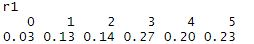
\includegraphics[scale=1]{probabilidad_condicionada2.JPG}\\
            \centering
            \caption{}
            
            
	\subsection{Bayes}
		\subsubsection{Teorema de Bayes                  }
		    El teorema de Bayes o regla de Bayes sea $B_1,..,B_n$ donde es una partición de de los posibles resultados, talque cada una de estas particiones la probabilidad sea distinta de cero (0)  Sea B un suceso cualquiera del que se conocen las probabilidades condicionales  $P(B|A)$. Entonces, la probabilidad $P(A|B)$ viene dada por la expresión:
		    \[
		    P(A/B)=\frac{P(B/A)P(A)}{P(B)}
		    \]
		    Donde cada probabilidad se define de la siguiente manera:
		    \begin{itemize}
		        \item P(A) son las probabilidades a priori
		        \item P$(B|A)$ es la probabilidad de $B$ en la hipótesis $A$
		        \item P$(A/B)$ son las probabilidades a posteriori. 
		    \end{itemize}
		    Ahora vamos a ejecutar un código para Bayes que funciona para cualquiera que sea el problema que se quiere ejecutar.
		    \begin{lstlisting}
		    print ("ingrese el porcentaje ")
                    porcentaje<-c(scan())
                    print ("ingrese la probabilidad ")
                    prob<-c(scan())
                    
                    funcionb<- function(porcentaje,prob){
                      suma <- 0.00
                      for(i in 1: length(porcentaje)){
                        suma<-suma+porcentaje[i]*prob[i]
                      
                      }
                      resta <- 0.00
                      probabilidad<-c()
                      for(i in 1:length(porcentaje)){
                        resta<-porcentaje[i]*prob[i]/suma
                        probabilidad<-c(probabilidad,resta)
                      }
                      return(probabilidad)
                    }
                    
                    print(funcionb(porcentaje,prob))

		    \end{lstlisting}\\
		Para probar que si funciona vamos a ejecutar un problema.
		
		Una empresa que fabrica celulares tiene dos maquinas A y B cada maquina fabrica el 60\% y 40\% de los celulares respectivamente y cada maquina tiene un 5\% y 10\% respectivamente de celulares defectuosos entonces ¿Cual es la probabilidad de que el celular haya sido fabricado por la maquina A sabiendo que es defectuoso?
		
		Usando el código simple vamos a digitar los porcentajes que van hacer \textbf{0.06} y\textbf{0.04} que son los porcentajes de fabricación de cada maquina, y después digitamos la probabilidad que es el defecto de cada maquina seran \textbf{0.05} y \textbf{0.10}
		nos va quedar como solución:\\
		    \centering
            
\includegraphics[scale=1]{Bayes.JPG}\\
            \centering
            \caption{}
            
            
	\subsection{Distribución binomial}
			Una distribución binomial es una distribución de probabilidad discreta que describe el número de éxitos al realizar en n experimentos independientes entre sí, acerca de una variable aleatoria.
			\\
			Se entiende como una serie de pruebas o
            ensayos en la que solo podemos tener 2
            resultados (sea éxito o fracaso), siendo el
            éxito nuestra variable aleatoria.
            \[P_{(x)}={n \choose r} p^{x}q^{n-x}\]
            \[P_{(x)}=\frac{n!}{(n-x)!x!}p^{x}q^{n-x}\]\\
            Donde:\\
            p= Probabilidad de éxito\\
            q= Probabilidad de fracaso\\
            x= Variable aleatoria\\
            n= Número de ensayos\\
            
            En R ya viene la función binomial y se puede usar de la siguiente manera \textbf{binom} pero no se usa así de simple se tiene que poner \textbf{dbinom} para usar la funcion binomial simple, probabilidad acumulada se usa \textbf{pbinom}, la inversa de la función de distribución, es decir, los percentiles \textbf{qbinom} y \textbf{rbinom} se usa para los valores binomiales generados.
            
            \textbf{Ejemplo}: Imaginemos que un 80\% de personas en el mundo han visto el partido  del final del último mundial de fútbol. Tras el evento, 4 amigos se reúnen a conversar. ¿Cuál es la probabilidad de que 3 de ellos hayan visto el partido?
            
            \begin{lstlisting}
                n <- 4
                p<- 0.8
                x <- 3
                dbinom(x,n,p)
            \end{lstlisting}
			nos va quedar como solución:\\
		    \centering
            
\includegraphics[scale=1]{binomial.JPG}\\
            \centering
            \caption{}
	\subsection{Distribución de Poisson}
			Esta distribución es una de las más importantes distribuciones de variable discreta, los experimentos que resultan en valores numéricos de una v.a $X$ y que representan el número de resultados durante un intervalo de tiempo dado o en una región específica frecuentemente se conocen como experimentos Poisson.
			\[
			P(x)=\frac{\mu^x \cdot e^{-\mu}}{x!}
			\]
			Veamos el siguiente ejemplo: Suponga que los accidentes de una calle siguen un proceso de Poisson con una taza de 2 accidentes por semana.\\
			\begin{itemize}
			    \item Hallar la probabilidad de que se comentan 5 accidentes durante la próxima semana.
			\end{itemize}\\
			Vamos a calcular mediante la función \textbf{pois} al igual que la función binomial tiene las mismas características,
			\textbf{dpois}, \textbf{ppois}, \textbf{qpois} y \textbf{rpois}
		    \textbf{dpois} es para la $x=X$ probabilidad acumulada se usa \textbf{ppois}, la inversa de la función de distribución, es decir, los percentiles \textbf{qpois} y \textbf{rpois} se usa para los valores binomiales generados.\\
		    Ahora para solucionar el ejemplo se usa el siguiente código:
		    \\
            Ejecutado el problema primero se halla lambda teniendo en cuenta que lambda se halla mediante, si 2 accidentes son por 1 (una) semana entonces por 5 accidentes en la siguiente semana entonces 
            \begin{center}
                $2\to 1 \\
                x\to 1
                $\\
                Entonces calcular la media y se encuentra que es dos, ese es el valor de lambda.
            \begin{lstlisting}
                x<-5
                lambda<-2
                dpois(x,lambda)
            \end{lstlisting}\\
            \end{center}
		    \centering
            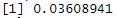
\includegraphics[scale=1]{poisson.JPG}\\
            \centering
            \caption{}
            
    \subsection{Distribución Z normal}
		En estadística y probabilidad se llama distribución normal, distribución de Gauss, distribución gaussiana o distribución de Laplace-Gauss, a una de las distribuciones de probabilidad de variable continua que con más frecuencia aparece en estadística y en la teoría de probabilidades.\\
		Una variable aleatoria continua, X, sigue una distribución normal de media $\mu$ y desviación típica $\sigma$, y se designa por N($\mu$,$\sigma$), si se cumplen las siguientes condiciones:
		\begin{itemize}
		    \item La variable puede tener valores desde ($-\infty,\infty$)
		    \item La función de densidad, es la expresión en términos de ecuación matemática de la curva de Gauss
		    \[
		        f(x)=\frac{1}{\sigma\sqrt{2\pi}}e^{-\frac{1}{2}(\frac{x-\mu}{\sigma})^2}
		    \]
		\end{itemize}
		Para estandarizar un valor de $X$:
		\[Z=\frac{x-\mu}{\sigma}\]
		Donde $\mu$ es la media y $\sigma$ es la distribución estándar.\\
		En R para hacer una distribución normal podemos usar la siguiente función \textbf{norm} al igual que las distribuciones de Poisson y binomial tiene:\\
		\textbf{dnorm}, \textbf{pnorm}, \textbf{qnorm} y \textbf{rnorm}.\\
		\textbf{dnorm} es para la $x=X$ probabilidad acumulada se usa \textbf{pnorm}, la inversa de la función de distribución, es decir, los percentiles \textbf{qnorm} y \textbf{rnorm} se usa para los valores binomiales generados.\\
		Vamos hacer el siguiente problema.\\
		 La temperatura durante septiembre está distribuida normalmente con media 18,7$\º$Cy desviación estándar 5$\º$C. Calcule la probabilidad de que la temperatura durante setiembre esté por debajo de 21$\º$C
		 \begin{lstlisting}
                x<-21
                media<-18.7
                desvia<-5
                pnorm(x,media,desvia)
            \end{lstlisting}\\
        Y la solución para el siguiente ejercicio es:\\
            \centering
            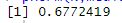
\includegraphics[scale=1]{normal.JPG}\\ \\
            \centering
            \caption{}
    \subsection{Intervalos de confianza}
        \subsubsection{Pruebas de hipótesis}
            Son procedimientos de decisión basado en datos que puedan producir una conclusión acerca de algún sistema científico.\\
            Una \textbf{hipótesis estadística} es una afirmación o conjetura acerca de una o más poblaciones.\\
            Tener en cuenta:
            \begin{itemize}
                \item Hipótesis nula  $H_0$: $\mu=\mu_0$; $\mu\leq\mu_0$; $\mu\geq\mu_0$
                \item Hipótesis Alternativa: $H_1:$ $\mu=\mu_1$; $\mu<\mu_1$; $\mu>\mu_1$; $\mu\neq\mu_1$
            \end{itemize}
            Para probar las hipótesis se tiene la prueba de normalidad de Kolmogorov-Smirnov, pruebas de variabilidad y pruebas de medias.
            \subsubsection{Prueba de normalidad}
            Los resultados de la prueba indican si usted debe rechazar o no puede rechazar la hipótesis nula de que los datos provienen de una población distribuida normalmente.
            \\ Vamos a usar la prueba de normalidad de Kolmogorov-Smirnov y de Shapiro Wilk
            \begin{itemize}
                \item \textbf{Prueba de normalidad de Kolmogorov-Smirnov}:\\
                Esta prueba compara la función de distribución acumulada empírica de los datos de la muestra con la distribución esperada si los datos fueran normales.
                Se va usar la el comando \textbf{lillie.test} hace el calculo de Kolmogorov-Smirnov mejorado para usar \textbf{lillie.test} tener en cuenta que toca instalar \textbf{nortest} y vamos a usar un ejemplo propio para eso, teniendo en cuenta que para Kolmogorov-Smirnov se usa para datos mayores a 50.
                \begin{lstlisting}
                set.seed(100)
                muestra<- rnorm(n=100,mean=170,sd=19)
                plot(density(muestra))
                library(nortest)
                lillie.test(muestra)$p.value
                
                \end{lstlisting}\\
                y su respuesta y gráfica serian las siguientes:\\
                \centering 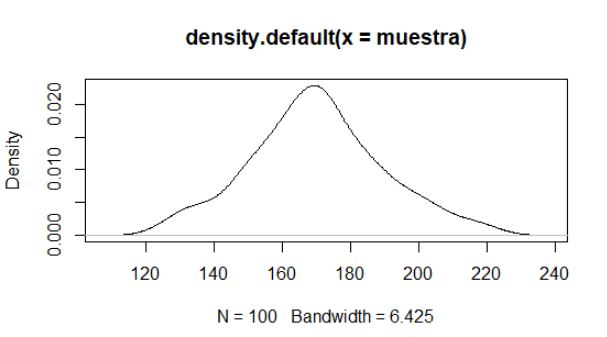
\includegraphics[scale=0.8]{ks_grafica1.jpeg}\\
                \centering
                \caption{}\\
                
                \centering
                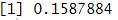
\includegraphics[scale=1]{ks1.JPG}\\ \\
                \centering
                \caption{respuesta Kolmogorov-Smirnov}
                
                \item \textbf{Prueba de normalidad Shapiro Wilk:}\\
                se usa para contrastar la normalidad de un conjunto de datos. Se plantea como hipótesis nula que una muestra $x_1,...,x_n$ proviene de una población normalmente distribuida\\
                \begin{lstlisting}
                    set.seed(50)
                    muestra<- rnorm(n=5,mean=10,sd=4)
                    plot(density(muestra))
                    library(nortest)
                    shapiro.test(muestra)$p.value
                    
                \end{lstlisting}\\
                \centering
                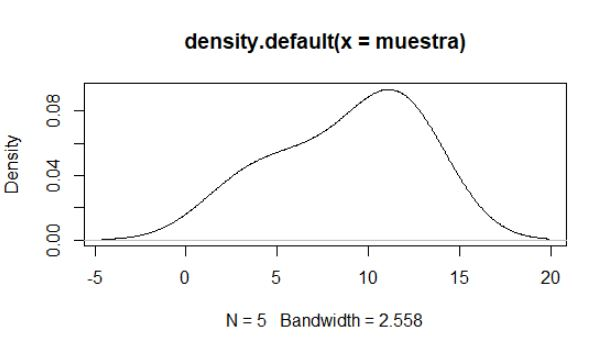
\includegraphics[scale=0.8]{ks_grafica.jpeg}\\
                \centering
                \caption{}\\
                
                \centering
                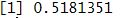
\includegraphics[scale=1]{ks.JPG}\\ \\
                \centering
                \caption{respuesta Shapiro Wilk}
            \end{itemize}
        \subsection{Prueba de varianza}
        Pruebas de hipótesis para una varianza es un procedimiento para juzgar si una propiedad que se supone cumple una población estadística es compatible con lo observado en una muestra de dicha población en este caso la varianza, para ello formularemos dos Hipótesis (llamada "Hipótesis Nula") y (llamada "Hipótesis Alternativa"), con ellas realizaremos una o más pruebas, para tratar de encontrar cual se debe rechazar.
        \\ cuando se trabaja con varianza se utiliza $chi^2$ que es una prueba de hipótesis que compara la distribución observada de los datos con una distribución esperada de los datos., por lo tanto nos vamos a concentrar en $chi^2$.\\
        Entonces vamos a R para usar crear una hipótesis para usar $chi^2$ en R es simplemente usar \textbf{chisq.test}.\\
        \begin{lstlisting}
        fumar=matrix(c(51,43,22,59,56,45,48,78,95),ncol=3,byrow = TRUE)
        colnames(fumar) = c("mucho","poco","medio")
        rownames(fumar) = c("actual","pasado","nunca")
        fumar=as.table(fumar)
        fumar
        chisq.test(fumar)
        \end{lstlisting}\\
        En el código hemos creado nuestra hipótesis de fumadores donde creamos una tabla de contingencia, datos inventados.\\
            \centering
            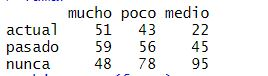
\includegraphics[scale=0.8]{chi.JPG}\\
            \centering
            \caption{}\\
        Y la respuesta de $chi^2$:\\
            \centering
            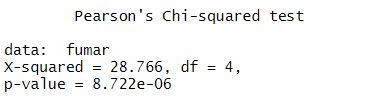
\includegraphics[scale=0.8]{chires.JPG}\\
            \centering
            \caption{}\\
    \subsection{Prueba de media}
    Se utiliza una prueba de una muestra para probar una afirmación con respecto a una media de una población única,en vez de estimar el valor de un parámetro, a veces se debe decidir si una afirmación relativa a un parámetro es verdadera o falsa.
    \\ En este caso Vamos a usar la prueba t que es muy buena que se utiliza cuando deseamos comparar dos medias (las cuentas se deben medir en una escala de intervalo o de cociente)\\
    Vamos A ejecutar un código en R de una prueba t student entonces para una prueba t student en E se necesita escribir el código con el siguiente código \textbf{t.test}.
        \begin{lstlisting}
        set.seed(10)
        x1 <- rnorm(100,10) 
        x2 <- rnorm(100,10.5) 
        test <- t.test(x1,x2)
        print(test)
        \end{lstlisting}\\
        Ejecutando el código.
            \centering
            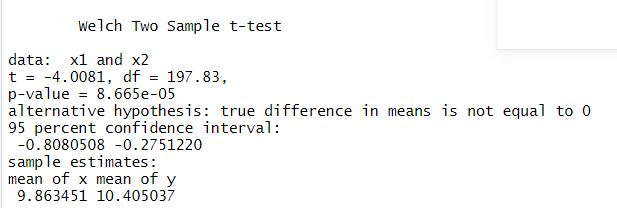
\includegraphics[scale=0.8]{t-s.JPG}\\
            \centering
            \caption{}\\
    Como el p-value es < 0.05 podemos afirmar que las muestras difieren en su media, es decir, las dos variables son diferentes con un gráfico de cajas se puede ayudar a interpretar este resultado,las medias se indican mediante un punto azul:\\   
    \begin{lstlisting}
        boxplot(x1,x2,names=c("X1","X2"))
        medias <- c(mean(x1),mean(x2))
        points(medias,pch=18,col="blue")
        \end{lstlisting}\\
            \centering
            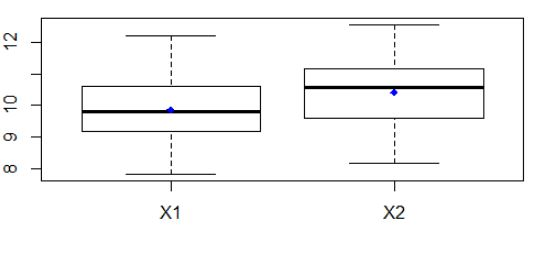
\includegraphics[scale=0.8]{grafica-t.JPG}\\
            \centering
            \caption{}\\


%%%%%%%%%%%%%%%%%%%%%%%%%%%%%%%%%%%%%%%%%%%%%%%%%%%%%%%%%%%

%%%%%%%%%%%%%%%%%%%%%%%%%%%%%%%%%%%%%%%%%%%%%%%%%%%%%%%%%%%%%%%%%%
\end{document}